\documentclass{article}
\usepackage[margin=3cm]{geometry}
\usepackage{graphicx}
\title{Combinatorial Optimization Project}
\author{Pierre-Louis Gstalter}
\begin{document}
\maketitle

\tableofcontents
\newpage

\subsubsection{Results}

\paragraph{{Structure
\texttt{graph}}{Structure graph}}

Here is the evolution of computational time for Dijkstra's on the
structure ``Graph'':

\begin{figure}
\centering
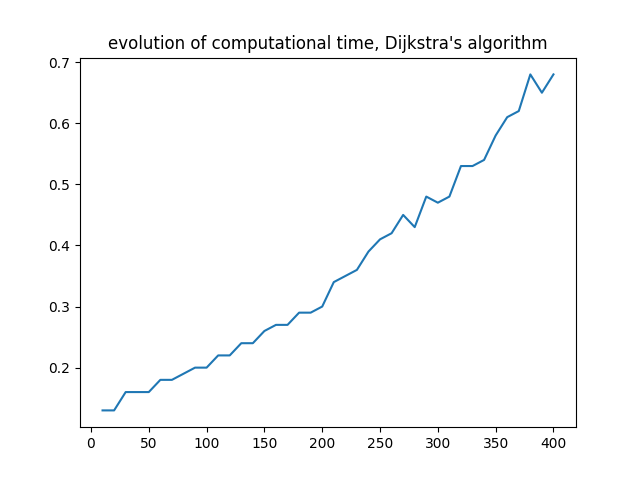
\includegraphics{ressources/dijkstra_res_graph.png}
\caption{dijkstra\_graph}
\end{figure}

Run on graphs of 10 to 400 nodes, at a given density.

And with different densities of arcs:

\begin{figure}
\centering
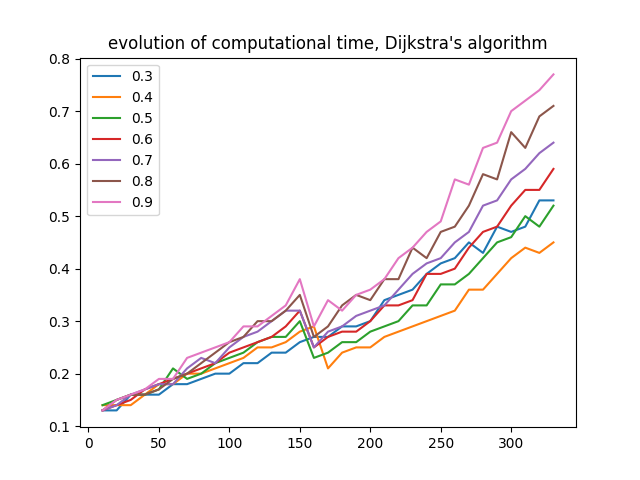
\includegraphics{ressources/dijkstra_res_graph_density.png}
\caption{variable\_density}
\end{figure}

\paragraph{{Strcture
\texttt{std\_graph}}{Strcture std\_graph}}

\begin{figure}
\centering
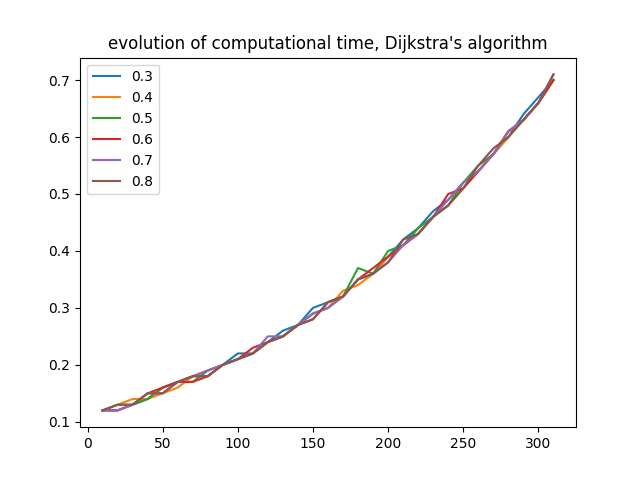
\includegraphics{ressources/dijkstra_density_std_graph.png}
\caption{std\_graph}
\end{figure}

It can be compared to the results obtained with \texttt{graph}:

\begin{figure}
\centering
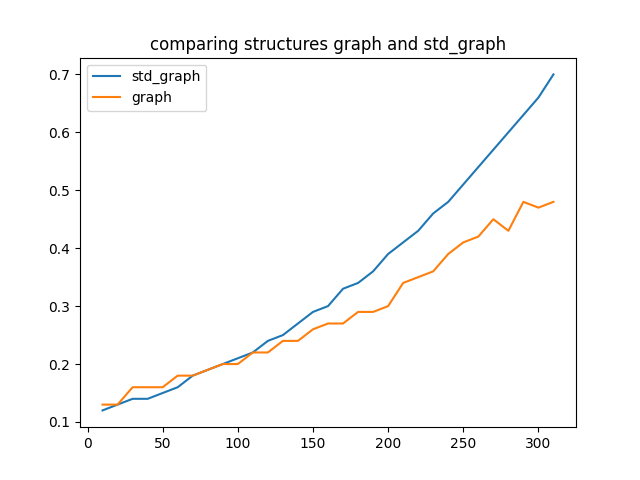
\includegraphics{ressources/comparing_graph__std_graph.png}
\caption{comparing}
\end{figure}

It can be seen that \texttt{std\_graph} tends to be slower as the number
of nodes (and hence arcs) increases. That's probably due to the fact
that the algorithm is very similar, but the data structure is larger
when the density is big.

Indeed, let's compare the size of the files containing \texttt{graph}
and \texttt{std\_graph} at two different densities:

\begin{figure}
\centering
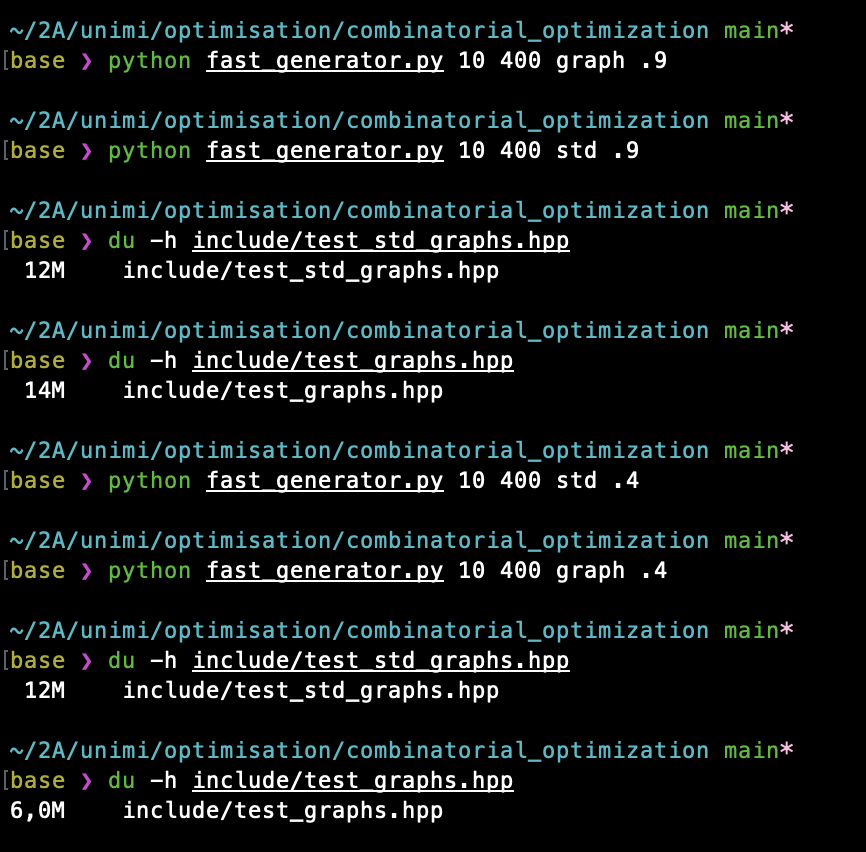
\includegraphics{ressources/spatial_comp.png}
\caption{comparing\_size}
\end{figure}

As expected, the files are very similar when the density is high.
\texttt{std\_graph} always has the same size and is hence more relevant
for \textbf{high densities}. On the contrary, when the density is low,
\texttt{std\_graph} contains lots of zeros, whereas \texttt{graph} only
keeps the \textbf{relevant} information. That's why \texttt{std\_graph}
takes up twice as much space on low densities.

\end{document}
